\documentclass[conference]{IEEEtran}
\IEEEoverridecommandlockouts
\usepackage{amsmath,amssymb,amsfonts}
\usepackage{algorithmic}
\usepackage{graphicx}
\usepackage{textcomp}
\usepackage{xcolor}
\usepackage{hyperref}
\usepackage{url}
\usepackage{float}
\usepackage{listings}

\definecolor{codegray}{rgb}{0.95,0.95,0.95}
\lstset{
  basicstyle=\ttfamily\footnotesize,
  backgroundcolor=\color{codegray},
  breaklines=true,
  frame=single,
  numbers=none,
  columns=fullflexible
}

\begin{document}

\title{Remote-Controlled Autonomous Tactical Rover for Human Detection\\
\large{CSE 4326 -- Final Project Report}}

\author{
\IEEEauthorblockN{Adnan Mohammad Salauddin}
\IEEEauthorblockA{ID: 011222361}
\and
\IEEEauthorblockN{Easmin Akter Tule}
\IEEEauthorblockA{ID: 011222177}
\and
\IEEEauthorblockN{Taki Tahmid}
\IEEEauthorblockA{ID: 011222172}
\and
\IEEEauthorblockN{Somaya Tabassum}
\IEEEauthorblockA{ID: 011222XXX}
\and
\IEEEauthorblockN{Shamim}
\IEEEauthorblockA{ID: 011222XXX}
}

\maketitle

\begin{abstract}
This report details the design and implementation of a Remote-Controlled Tactical Rover built using a Raspberry Pi and an Arduino Nano. The Raspberry Pi manages computer vision (human detection using a YOLOv8 model), runs a Flask web server for the remote control dashboard, and drives the chassis motors. The Arduino Nano operates the scanning turret and launcher. The two boards communicate over a one-way serial link. The system has two main operating modes: autonomous mode, where the rover drives forward and fires when a human is detected, and manual mode, allowing the operator to steer from the web dashboard. An emergency stop is also provided. The prototype shows that a basic tactical rover can be built using affordable, off-the-shelf components.
\end{abstract}

\begin{IEEEkeywords}
tactical robotics, Raspberry Pi, Arduino Nano, YOLOv8, autonomous human detection, remote-controlled rover, computer vision, Flask, serial communication
\end{IEEEkeywords}

\section{Introduction}
Autonomous ground robots are widely used in defense, but their development is limited in Bangladesh due to high costs. This project demonstrates that a working tactical rover prototype can be built on a low budget using a Raspberry Pi and an Arduino Nano instead of expensive specialized hardware. Our goal was to see if a dual-controller setup can handle real-time human detection and remote control while keeping the firing mechanism safe and simple.

The report covers our hardware selection, the software architecture on both controllers, dashboard features, and testing results.

\section{Project Motivation}
We designed this project with five key objectives in mind:
\begin{itemize}
    \item \textbf{Safety:} Keep operators away from danger by using remote control over Wi-Fi.
    \item \textbf{Precision:} Use AI (YOLOv8) to help detect human targets accurately.
    \item \textbf{Low Cost:} Use decoupled, cheap hardware (Raspberry Pi and Arduino Nano) so the system is cheap to build and repair.
    \item \textbf{Local Prototyping:} Build local capacity in Bangladesh for tactical robotics using off-the-shelf components.
    \item \textbf{Safety Override:} Keep a manual control override and an emergency stop active at all times.
\end{itemize}

\section{System Architecture}
The rover is split into two subsystems. The Raspberry Pi controls driving and runs the computer vision, while the Arduino Nano controls the turret and launcher. 

For safety, the Pi never controls the launcher directly. Instead, it sends a single serial character ('F') to the Arduino when a human is detected in autonomous mode. This decoupled setup keeps the firing mechanism independent and safe.

The auto mode follows this simple path (shown in Fig.~\ref{fig:flowchart}):
\begin{enumerate}
    \item The camera captures frames.
    \item The YOLOv8 model runs on the Pi to check for humans (confidence $> 0.6$).
    \item If a human is detected, the Pi stops the motors and sends 'F' to the Arduino.
    \item The Arduino Nano executes the firing sequence.
\end{enumerate}

\begin{figure}[H]
\centering
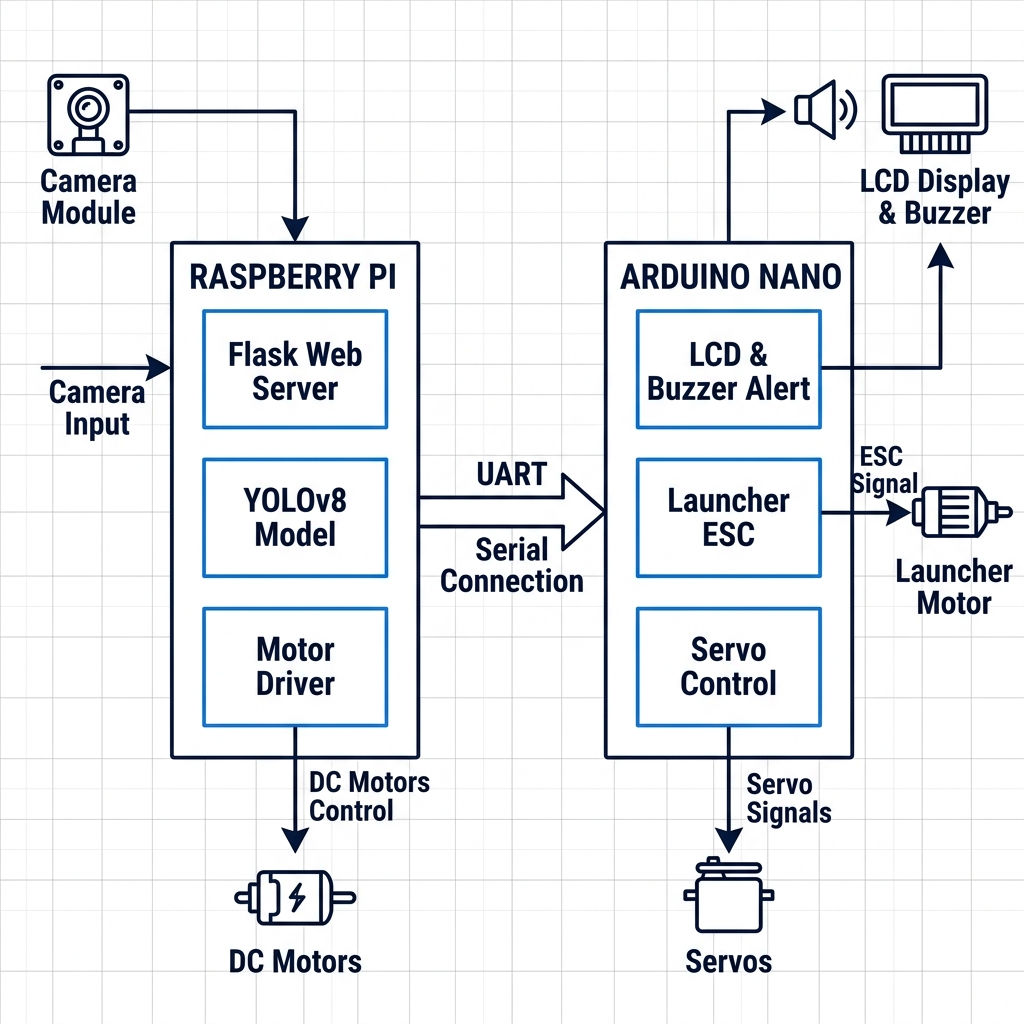
\includegraphics[width=0.95\linewidth]{fig_block_diagram.png}
\caption{High-level system block diagram showing the Raspberry Pi (vision, drive control, Flask web server) and the Arduino Nano (turret scanning, fire sequence), linked by a serial UART connection. \textit{[Placeholder -- insert system block diagram here.]}}
\label{fig:block}
\end{figure}

\begin{figure}[H]
\centering
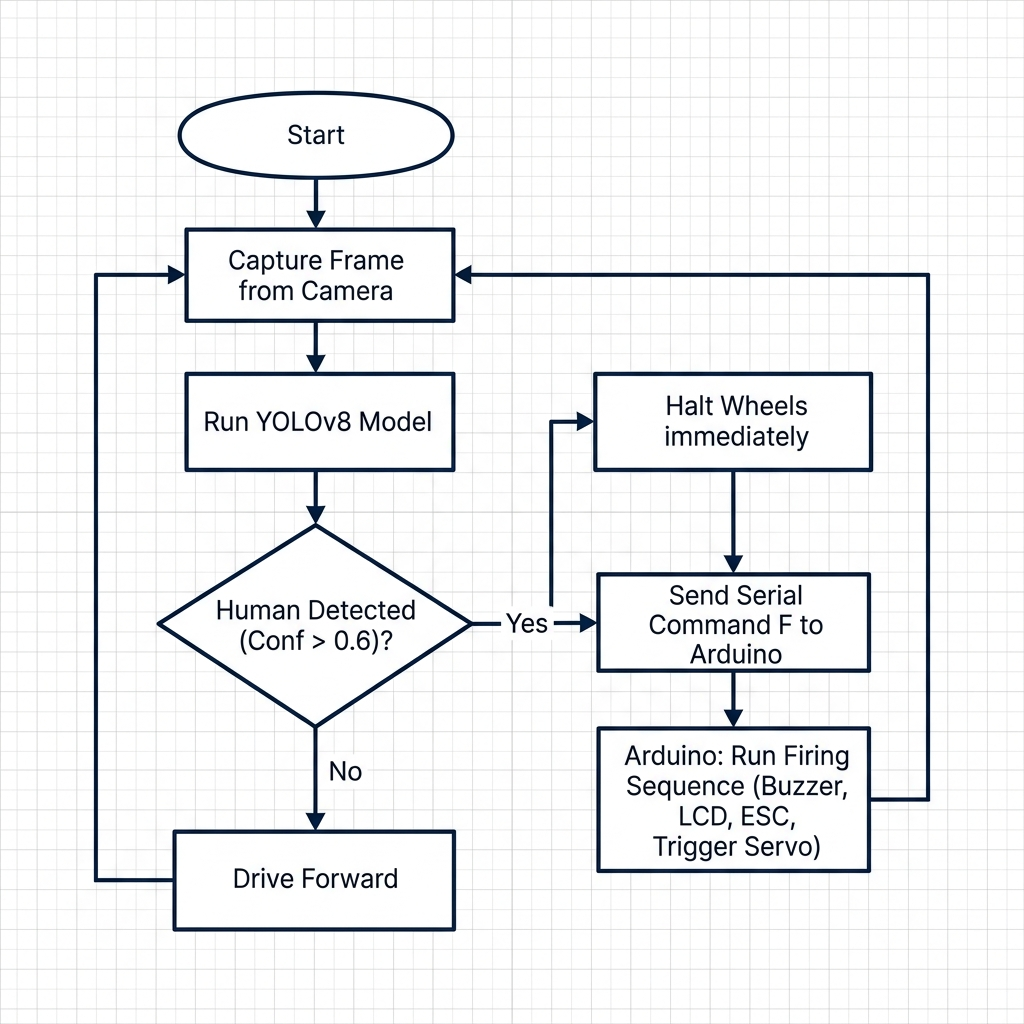
\includegraphics[width=0.85\linewidth]{fig_flowchart.png}
\caption{AUTO-mode operation flow: camera capture $\rightarrow$ YOLOv8 human detection $\rightarrow$ stop and send fire command over serial $\rightarrow$ Arduino executes fire sequence. \textit{[Placeholder -- insert flowchart diagram here.]}}
\label{fig:flowchart}
\end{figure}

\section{Hardware Design}
The major hardware components are listed below:
\begin{itemize}
    \item \textbf{Raspberry Pi:} Main controller. Runs the Flask web server, processes YOLOv8n, and drives the DC motors via GPIO pins.
    \item \textbf{2WD Chassis:} A basic differential-drive chassis for movement.
    \item \textbf{Turret Subsystem:} Uses an Arduino Nano to control four servos and a flywheel motor ESC. Servos 1, 2, and 4 handle scanning (horizontal and vertical). Servo 3 triggers the launcher. An LCD and buzzer provide local alerts.
\end{itemize}

Figures \ref{fig:piunit}, \ref{fig:turretunit}, \ref{fig:lcdstatus}, and \ref{fig:wiring} show the physical units and wiring. Table~\ref{tab:hardware} summarizes the components.

\begin{figure}[H]
\centering
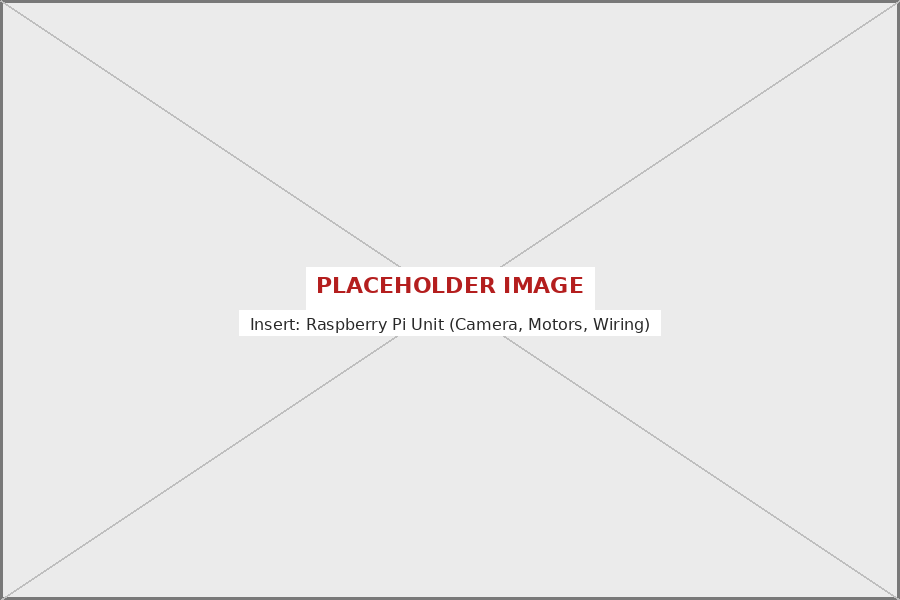
\includegraphics[width=0.95\linewidth]{fig_pi_unit.png}
\caption{Raspberry Pi unit showing the camera module, drive motor wiring, and main control board. \textit{[Placeholder -- insert photo of the Raspberry Pi and drive subsystem here.]}}
\label{fig:piunit}
\end{figure}

\begin{figure}[H]
\centering
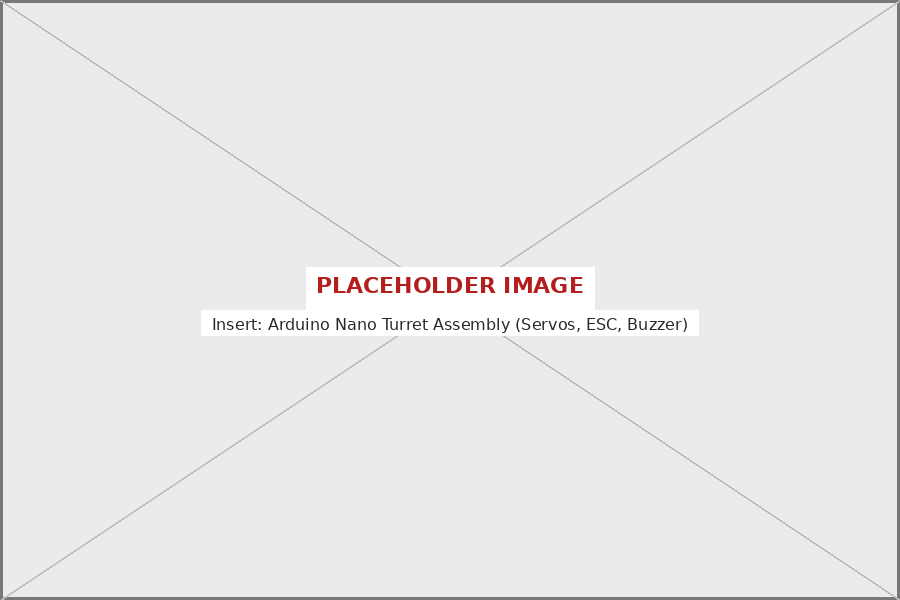
\includegraphics[width=0.95\linewidth]{fig_turret_unit.png}
\caption{Arduino Nano turret assembly showing the four servos, ESC/launcher motor, buzzer, and LCD display. \textit{[Placeholder -- insert close-up photo of the turret assembly here.]}}
\label{fig:turretunit}
\end{figure}

\begin{figure}[H]
\centering
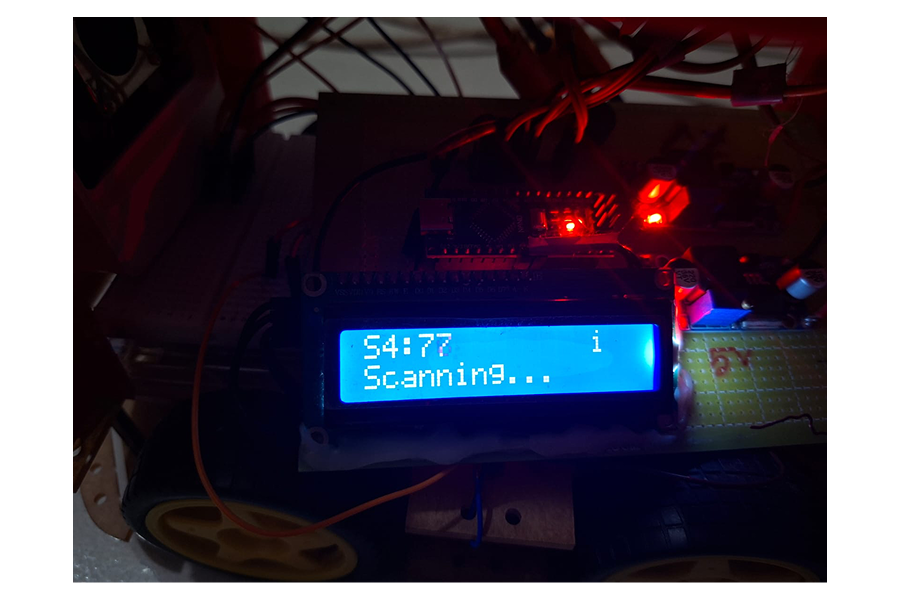
\includegraphics[width=0.95\linewidth]{fig_lcd_status.png}
\caption{LCD status display showing a live status message during the fire sequence (e.g., ``TARGET LOCKED'' / ``FIRE!!!''). \textit{[Placeholder -- insert close-up photo of the LCD display here.]}}
\label{fig:lcdstatus}
\end{figure}

\begin{figure}[H]
\centering

\includegraphics[width=0.95\linewidth]{fig_wiring.png}
\caption{Serial (UART) wiring between the Raspberry Pi and the Arduino Nano, along with motor and GPIO connections. \textit{[Placeholder -- insert wiring photo or diagram here.]}}
\label{fig:wiring}
\end{figure}

\begin{table}[H]
\caption{Hardware Components and Roles}
\label{tab:hardware}
\centering
\begin{tabular}{|p{2.1cm}|p{2.4cm}|p{2.6cm}|}
\hline
\textbf{Component} & \textbf{Role} & \textbf{Interface} \\
\hline
Raspberry Pi & Vision, web server, drive control & Camera (CSI), GPIO, Serial \\
\hline
Pi Camera & Video capture for AI \& streaming & CSI port \\
\hline
2$\times$ DC Motors & Differential drive & GPIO 17, 27, 22, 23 \\
\hline
Arduino Nano & Turret scanning \& firing & Serial (RX/TX) \\
\hline
Servo 1 / Servo 4 & Horizontal scan sweep & Pins D3 / D4 \\
\hline
Servo 2 & Vertical nod sweep & Pin D5 \\
\hline
Servo 3 & Fire-trigger actuator & Pin D6 \\
\hline
ESC + Launcher & Firing flywheel/launcher & Pin D10 \\
\hline
Buzzer & Audible fire alert & Pin D11 \\
\hline
16x2 I2C LCD & Status display & I2C (addr. 0x27) \\
\hline
\end{tabular}
\end{table}

\section{Software Implementation}
\subsection{Raspberry Pi Program}
The Pi runs a Flask application. A background thread processes camera frames, runs YOLOv8n at 256px resolution, and checks for humans. Flask routes handle remote driving inputs and video streaming. Listing~\ref{lst:ai_loop} shows the decision logic.

\begin{lstlisting}[caption={Core AUTO/MANUAL decision logic.}, label={lst:ai_loop}, language=Python]
if mode == "auto" and not emergency_stop:
    if human_detected:
        stop()
        fire()      # sends 'F' over serial
    else:
        forward()
elif mode == "manual" and not emergency_stop:
    apply_command()  # last manual key

if emergency_stop:
    stop()
\end{lstlisting}

\subsection{Arduino Nano Firmware}
The Arduino Nano sweeps the scanning servos during idle. When it receives 'F' over UART, it runs the fire sequence (buzz, LCD status, spin up flywheel, trigger servo sweep, and reset). Listing~\ref{lst:fire_seq} shows the code.

\begin{lstlisting}[caption={Fire sequence executed on the Arduino Nano.}, label={lst:fire_seq}, language=C++]
void fireSequence() {
  digitalWrite(BUZZER_PIN, HIGH);
  lcd.print("!! HUMAN !! DETECTED");

  esc.writeMicroseconds(ESC_MAX_US);  // spin up launcher
  servo3.write(0);                     // trigger
  delay(800);
  servo3.write(180);                   // reset trigger
  esc.writeMicroseconds(ESC_MIN_US);   // stop launcher

  digitalWrite(BUZZER_PIN, LOW);
  lcd.print("FIRE COMPLETE / Scanning...");
}
\end{lstlisting}

\subsection{Communication}
We use a simple one-way serial link (UART) from the Pi to the Arduino to send firing commands. No feedback is returned to the Pi, keeping the protocol simple.

\section{Control Interface}
The operator interacts with the rover through a web dashboard (Fig.~\ref{fig:dashboard}) served by Flask. The dashboard provides:
\begin{itemize}
    \item Live camera stream from the Pi.
    \item AUTO and MANUAL mode toggles.
    \item Emergency STOP button.
    \item Speed presets and manual drive controls.
\end{itemize}

\begin{figure}[H]
\centering
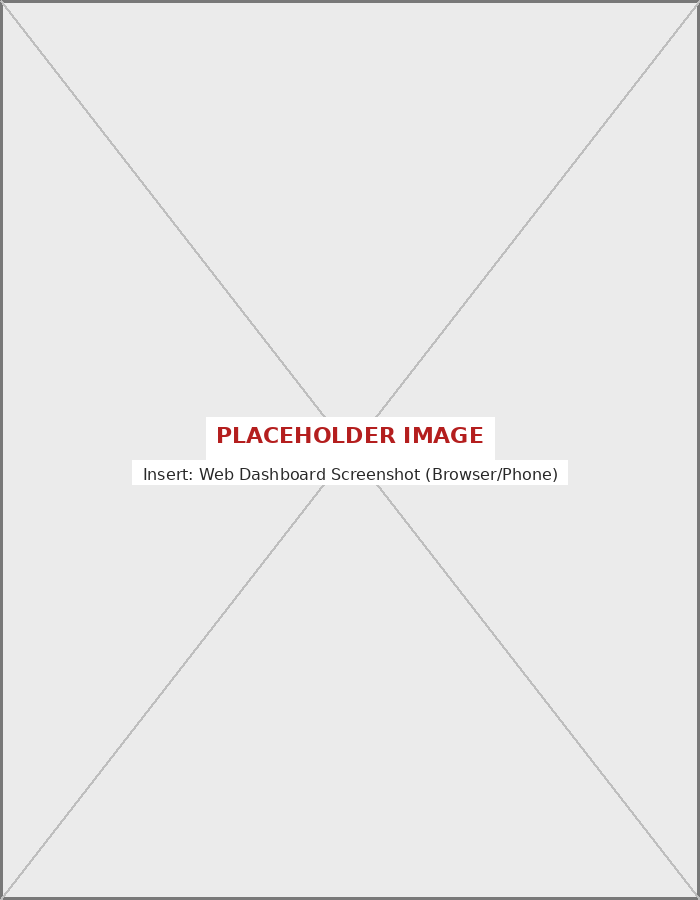
\includegraphics[width=0.7\linewidth]{fig_dashboard.png}
\caption{Browser-based control dashboard showing the live camera feed, AUTO/MANUAL/STOP buttons, and speed controls. \textit{[Placeholder -- insert screenshot of the web dashboard here.]}}
\label{fig:dashboard}
\end{figure}

\begin{figure}[H]
\centering
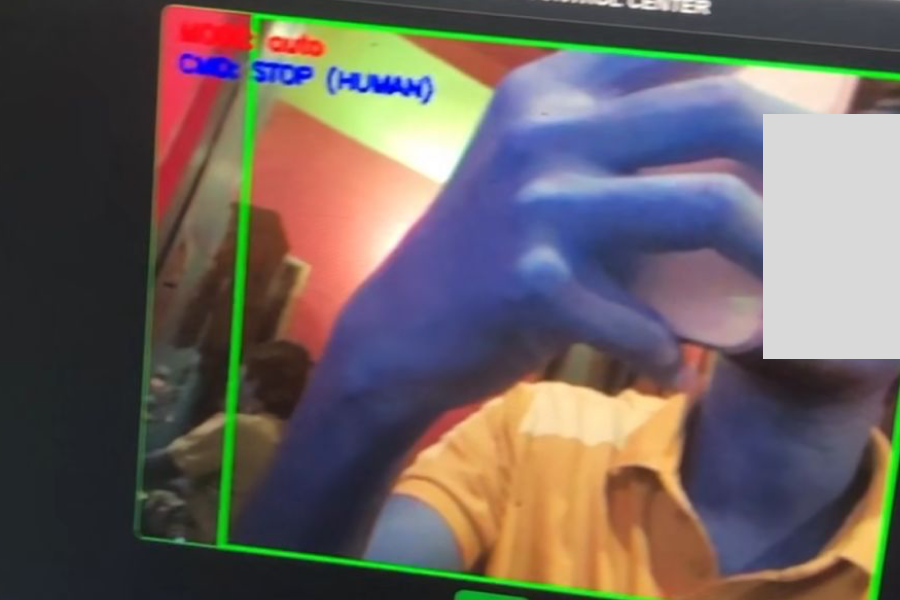
\includegraphics[width=0.95\linewidth]{fig_detection_demo.png}
\caption{Sample YOLOv8 detection output on the live camera feed, showing a person correctly classified above the confidence threshold. \textit{[Placeholder -- insert screenshot of YOLO detection output here.]}}
\label{fig:detection}
\end{figure}

\section{System Demonstration}
The complete physical prototype integrates the Pi driving base and the Arduino turret as shown in Fig.~\ref{fig:overview}.

\begin{figure}[H]
\centering
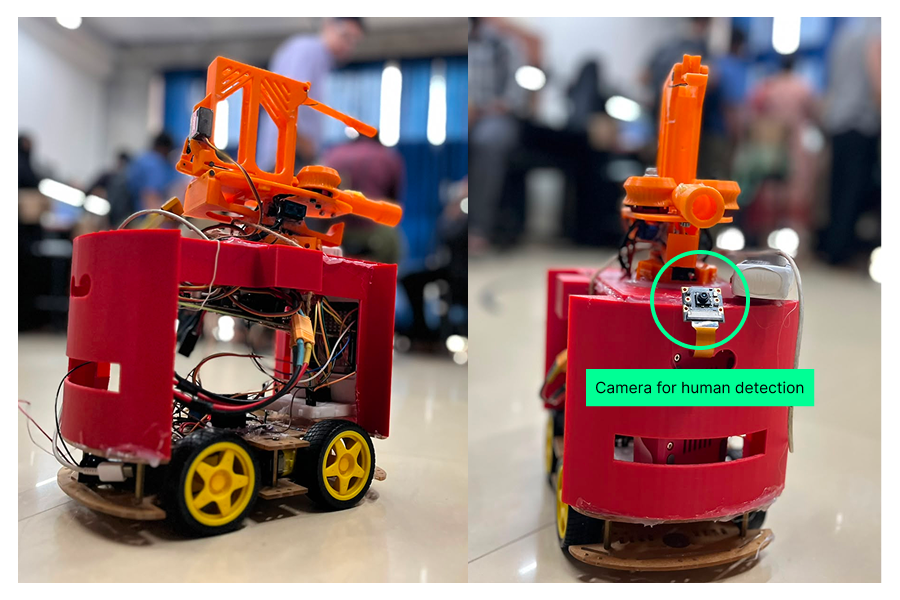
\includegraphics[width=0.95\linewidth]{fig_system_overview.png}
\caption{Complete assembled Remote-Controlled Tactical Rover prototype, integrating the Raspberry Pi drive unit and Arduino Nano turret. \textit{[Placeholder -- insert full system photo here.]}}
\label{fig:overview}
\end{figure}

\section{Results and Discussion}
Testing showed the following:
\begin{itemize}
    \item The dual-controller setup worked reliably with fast serial communication.
    \item The YOLOv8 model detected humans with low latency.
    \item Switching between AUTO and MANUAL modes was instant.
    \item The emergency stop halted the motors immediately.
\end{itemize}

\section{Limitations}
A few key limitations were identified:
\begin{itemize}
    \item YOLOv8n at 256px resolution is sensitive to lighting and distance.
    \item A single-frame detection is used, which can cause false alarms.
    \item The web interface and serial link are unencrypted.
    \item The communication is one-way (no feedback from Arduino).
    \item There are no sensors for obstacle avoidance.
\end{itemize}

\section{Conclusion and Future Work}
This project shows a low-cost tactical rover prototype is viable using basic components. Future updates will focus on:
\begin{enumerate}
    \item Requiring multiple frames of detection to prevent false fires.
    \item Adding sonar/depth sensors for obstacle avoidance.
    \item Securing the web dashboard and serial communication.
    \item Adding bidirectional telemetry.
\end{enumerate}

\section*{Project Resources}
\begin{itemize}
    \item \textbf{GitHub Repository:} \url{https://github.com/takitahmid20/tactical-robotics.git}
    \item \textbf{Video Demonstration:} \url{https://drive.google.com/drive/folders/1rty6dcJoT33Ydw6i4qH2ZektXo1Qzls9?usp=sharing}
\end{itemize}

\section*{Acknowledgment}
The authors thank the course instructor for guidance throughout the design and development of this project as part of CSE 4326.

\end{document}
